%!TEX root = htm.tex
\section{Hybrid transactional memory (HyTM)}
\label{sec:hytm}
%
In this section, we adopt the formal model of HyTMs originally proposed in \cite{htmdisc15}.

\vspace{1mm}\noindent\textbf{Transactional memory (TM).} 
A \emph{transaction} is a sequence of \emph{transactional operations}
(or \emph{t-operations}), reads and writes, performed on a set of \emph{transactional objects} 
(\emph{t-objects}). 
A TM \emph{implementation} provides a set of
concurrent \emph{processes} with deterministic algorithms that implement reads and
writes on t-objects using  a set of \emph{base objects}.
% More precisely, for each transaction $T_k$, a TM implementation must support the following t-operations: 
% $\mathit{read}_k(X)$, where $X$ is a t-object, that returns a value in
% a domain $V$
% or a special value $A_k\notin V$ (\emph{abort}),
% $\mathit{write}_k(X,v)$, for a value $v \in V$,
% that returns $\mathit{ok}$ or $A_k$, and
% $\mathit{tryC}_k$ that returns $C_k\notin V$ (\emph{commit}) or $A_k$.
% Additionally, we assume that a transaction $T_k$
% may perform a $\mathit{start_k}$ that is the first t-operation performed by $T_k$ prior to invoking any $\mathit{read}_k$ or $\mathit{write}_k$.

\vspace{1mm}\noindent\textbf{Configurations and executions.} 
A \emph{configuration} of a TM implementation specifies the state of each base object and each process. 
In the \emph{initial} configuration, each base object has its initial value and each process is in its initial state. 
An \emph{event} (or \emph{step}) of a transaction invoked by some process is an invocation of a t-operation, 
a response of a t-operation, or an atomic \emph{primitive} operation applied to base object along with its response. 
%An event $e$ is \emph{applicable} to a configuration $C$ if $e$ can legally be applied to $C$. 
%Applying an event $e$ to a configuration $C$ results in another configuration $C' = e(C)$.
An \emph{execution fragment} is a (finite or infinite) sequence of events $E = e_1,e_2,\dots$. 
%$E$ is applicable to a configuration $C$ if $e_1$ is applicable to $C$, $e_2$ is applicable to $e_1(C)$, 
%and so forth. 
An \emph{execution} of a TM implementation $\mathcal{M}$ is an
execution fragment where, informally, each event respects the
specification of base objects and the algorithms specified by $\mathcal{M}$.

We consider the dynamic programming model: the \emph{read set} (resp., the \emph{write set}) of a transaction $T_k$ in an execution $E$,
denoted $\Rset_E(T_k)$ (resp., $\Wset_E(T_k)$), is the set of t-objects that $T_k$ attempts to read (and resp. write) 
by issuing a t-read (resp., t-write) invocation in $E$ (for brevity, we sometimes 
omit the subscript $E$ from the notation).

For any finite execution $E$ and execution fragment $E'$, $E\cdot E'$ denotes the concatenation of $E$ and $E'$,
and we say that $E\cdot E'$ is an \emph{extension}
of $E$.
%Let $E$ be an execution fragment.
For every transaction identifier $k$,
$E|k$ denotes the subsequence of $E$ restricted to events of
transaction $T_k$.
% If $E|k$ is non-empty,
% we say that $T_k$ \emph{participates} in $E$,
% and let $\txns(E)$ denote the set of transactions that participate in $E$.
Two executions $E$ and $E'$
are \emph{indistinguishable} to a set $\mathcal{T}$ of transactions, if
for each transaction $T_k \in \mathcal{T}$, $E|k=E'|k$.
\trevor{where is $\txns(E)$ defined?}
A transaction $T_k\in \txns(E)$ is \emph{complete in $E$} if
$E|k$ ends with a response event.
The execution $E$ is \emph{complete} if all transactions in $\txns(E)$
are complete in $E$.
A transaction $T_k\in \txns(E)$ is \emph{t-complete} if $E|k$
ends with $A_k$ or $C_k$; otherwise, $T_k$ is \emph{t-incomplete}.

We assume that base objects are accessed with \emph{read-modify-write} (rmw) primitives. 
% A rmw primitive $\langle g,h \rangle$ applied to a base object 
% atomically updates the value of the object with a new value, which is
% a function $g(v)$ of the old value $v$, and returns a response $h(v)$.
%A rmw primitive is \emph{trivial} if it never affects the value of a
%base object, otherwise it is \emph{nontrivial}.
A rmw primitive event on a base object is \emph{trivial} if, in any configuration, its application
does not change the state of the object. 
Otherwise, it is called \emph{nontrivial}.
Events $e$ and $e'$ of an execution $E$  \emph{contend} on a base
object $b$ if they are both primitives on $b$ in $E$ and at least 
one of them is nontrivial.

\vspace{1mm}\noindent\textbf{Hybrid transactional memory executions.}
We now describe the execution model of a \emph{Hybrid transactional memory (HyTM)} implementation.
In our HyTM model, shared memory configurations may be modified by accessing base objects via two kinds of
primitives: \emph{direct} and \emph{cached}.
(i) In a direct access, the rmw primitive operates on the memory state:
the direct-access event atomically reads the value of the object in
the shared memory and, if necessary, modifies it.
(ii) In a cached access performed by a process $i$, the rmw primitive operates on the \emph{cached}
state recorded in process $i$'s \emph{tracking set} $\tau_i$. 

More precisely, $\tau_i$ is a set of triples $(b, v, m)$ where $b$ is a base object identifier, $v$ is a value, 
and $m \in \{\shared, \exclusive\}$ is an access \emph{mode}. 
The triple $(b, v, m)$ is added to the tracking set when $i$ performs a cached
rmw access of $b$, where $m$ is set to $\exclusive$ if the access is
nontrivial, and to $\shared$ otherwise.  
%we assume that there exists some constant $\TS$ (representing the size of the L1 cache)
% such that the condition $|\tau_i| \leq \TS$ must always hold; this
% condition will be enforced by our model.
A base object $b$ is \emph{present} in $\tau_i$ with mode $m$ if $\exists v, (b,v,m) \in \tau_i$.

% A trivial (resp.\ nontrivial) 
% cached primitive $\langle g,h \rangle$ applied to $b$ 
% by process $i$ 
% checks whether $b$ is present in exclusive
% (resp.\ any) mode in $\tau_j$ 
% for any $j\neq i$. If so, $\tau_i$ is set to $\emptyset$ and the
% primitive returns $\bot$. 
% %
% Otherwise, the triple $(b, v, \shared)$ (resp. $(b, g(v), \exclusive)$)
% is added to $\tau_i$,  where $v$ is the most recent cached value of $b$ in $\tau_i$
% (in case $b$ was previously accessed by $i$ within the current
% hardware transaction) or the value of $b$ in the current
% memory configuration, and finally $h(v)$ is returned.
%

\vspace{1mm}\noindent\textbf{Hardware aborts.}
A tracking set can be \emph{invalidated} by a concurrent process: 
if, in a configuration $C$ where  $(b,v,\exclusive)\in\tau_i$
(resp., $(b,v,\shared)\in\tau_i)$,  a process $j\neq i$ applies any primitive 
(resp., any \emph{nontrivial} primitive) to $b$, then $\tau_i$ becomes
\emph{invalid} and any subsequent event invoked by $i$
sets $\tau_i$ to $\emptyset$ and returns $\bot$. We refer to this event as a \emph{tracking set abort}.
% Note that hardware transactions may also abort spuriously, or because of unsupported operations~\cite{Rei12}, or due to \emph{capacity} aborts. 
% Since modelling these aborts will not affect our results, except make for a more cumbersome presentation, we only consider capacity aborts in this paper. 

Any transaction $T_k \in \ms{txns}(E)$ that performs at least one cached access necessarily performs a \emph{cache-commit} primitive as the last event of $E|k$. 
\trevor{why can't it be a user-requested abort? what if, e.g., you are implementing TLE, so you read a lock state and see that it is locked, and want to abort?}
A \emph{cache-commit} primitive issued by process $i$ with
a valid $\tau_i$ does the following: for each base object $b$ such that $(b,v,\exclusive) \in \tau_i$, the value of $b$ in $C$ is updated to $v$. 
\trevor{what is $C$? the configuration just before the \textit{cache-commit} primitive?}
Finally, $\tau_i$ is set to $\emptyset$ and the primitive 
returns $\textit{commit}$. 

\vspace{1mm}\noindent\textbf{Slow-path and fast-path transactions.}
We partition HyTM transactions into \emph{fast-path transactions} and \emph{slow-path transactions}.
A slow-path transaction models a regular software transaction.
An event of a slow-path transaction is either an invocation or response of a t-operation, or
a direct rmw primitive on a base object. 
A fast-path transaction essentially encapsulates a hardware transaction. Specifically, in any execution $E$,
we say that a transaction $T_k\in \ms{txns}(E)$ is a fast-path transaction if $E|k$ contains at least one cached event.
An event of a \emph{hardware transaction} includes series of direct trivial accesses and at least one cached access
followed by a \emph{cache-commit} primitive.

We assume that a fast-path transaction $T_k$ returns $A_k$
as soon an underlying cached primitive or \emph{cache-commit} returns $\bot$.
This implies the following observation:
%
\begin{observation}
\label{ob:traborts}
%
Let $T_k \in \ms{txns}(E)$ be any t-incomplete transaction executed by process $i$, where $(b,v,\exclusive)\in\tau_i$ (resp., $(b,v,\shared)\in\tau_i$) after execution $E$, and $e$ be any event (resp., nontrivial event) that some process $j\neq i$ is poised to apply after $E$.
The next event of $T_k$ in any extension of $E\cdot e$ is $A_k$.
%
%For any t-incomplete transaction $T_k \in \ms{txns}(E)$ executed by process $i$ and $(b,v,\exclusive)\in\tau_i$ (and resp. $(b,v,\shared)\in\tau_i$) after execution $E$
%and let $e$ be any event (and resp. nontrivial event) that some process $j\neq i$ is poised to apply after $E$, then the next event of $T_k$ in any extension of $E\cdot e$
%is $A_k$.
\end{observation}
%
\vspace{1mm}\noindent\textbf{Non-cached reads inside fast-path.}
Note that we specifically allow hardware transactions to perform reads without adding the corresponding base object to
the process's tracking set, thus modelling the non-speculative accesses inside hardware allowed by 
IBM Power8 architectures. We remark that Intel's HTM does not support this feature: an event of a hardware transaction
does not include any direct access.

%
\vspace{1mm}\noindent\textbf{HyTM properties.}
\trevor{reading here}
Throughout this paper, we consider the TM-correctness property of \emph{opacity}~\cite{tm-book}: an execution
$E$ is opaque if there exists a \emph{legal} sequential execution $S$ equivalent to some t-completion of $E$
that respects the \emph{real-time ordering} of transactions in $E$.

We also assume a weak TM-liveness property for t-operations in this paper: every t-operation returns a matching
response within a finite number of its own steps if running step-contention free from a \emph{quiescent} configuration,
\emph{i.e.}, a configuration in which every transaction is t-complete.

Algorithms and lower bounds presented in this paper concern HyTMs that provide \emph{invisible reads}: t-read operations do not perform
nontrivial primitives in any execution.
%
%
% \begin{figure*}[!ht]
% \begin{center}
% 	\subfloat[\label{sfig:ob-01}]{\scalebox{0.5}[0.5]{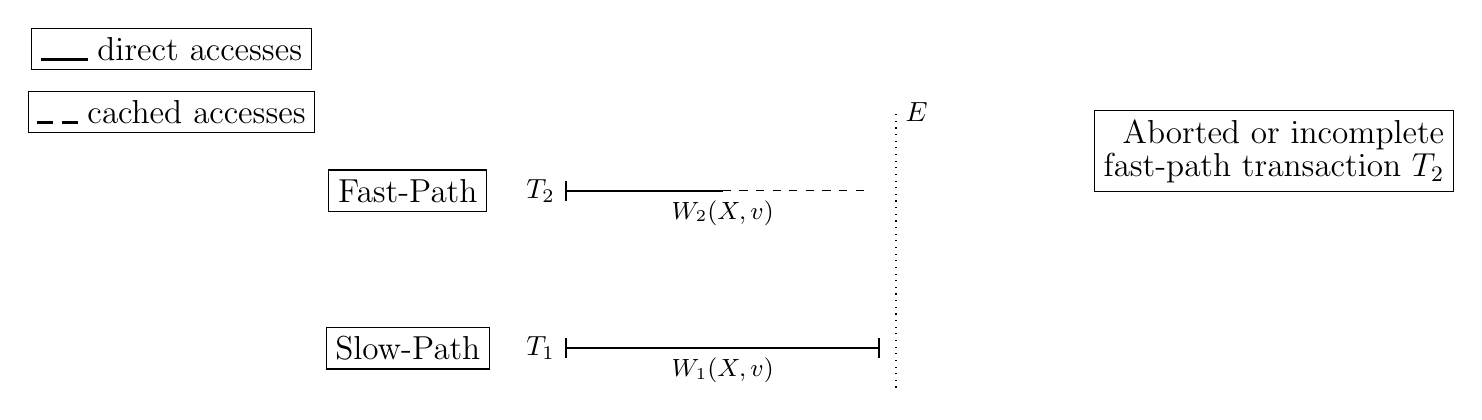
\begin{tikzpicture}
\node (w2) at (10,0) [] {};
\node (w1) at (10,-2) [] {};
\node (w3) at (18,-2) [] {};


\draw (w2) node [below] {\small {$W_2(X,v)$}};

\draw (w1) node [below] {\small {$W_1(X,v)$}};
%\draw (w1) node [below] {\tiny {$T_1$ commits}};

\node[draw,align=left] at (6,0) {{\large Fast-Path}};
\node[draw,align=left] at (6,-2) {{\large Slow-Path}};

\begin{scope}   
\draw [|-,thick] (8,0) node[left] {$T_2$} to (10,0);
\draw [-,dashed] (10,0) to (11.8,0);
\draw [|-|,thick] (8,-2) node[left] {$T_1$} to (12,-2);
\draw [-,dotted] (12.2,-2.5)  to (12.2,1) node[right] {$E$};
\end{scope}
%
\node[draw,align=right] at (17,.5) {\large {Aborted or incomplete}\\ {\large fast-path transaction $T_2$}};
%
\node[draw,align=right] at (3,1.8) {\rule{6mm}{1pt} \large {direct accesses}};
\node[draw,align=right] at (3,1) {\rule{2mm}{1pt} \rule{2mm}{1pt} \large{cached accesses}};

%
\end{tikzpicture}
}}
% 	\hspace{10mm}
% 	\subfloat[\label{sfig:ob-02}]{\scalebox{0.5}[0.5]{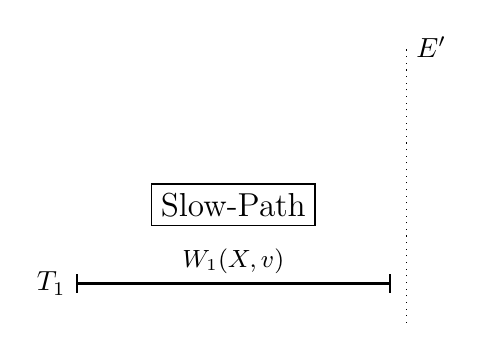
\begin{tikzpicture}

\node (w1) at (11,-2) [] {};


\draw (w1) node [above] {\small {$W_1(X,v)$}};
%\draw (w1) node [below] {\tiny {$T_1$ commits}};

\node[draw,align=left] at (11,-1) {{\large Slow-Path}};

\begin{scope}   
\draw [|-|,thick] (9,-2) node[left] {$T_1$} to (13,-2);
\draw [-,dotted] (13.2,-2.5)  to (13.2,1) node[right] {$E'$};
\end{scope}
%
%
\end{tikzpicture}
}}
% 	 
% \end{center}
% \caption{
% \label{fig:ob1}
% Execution $E$ in Figure~\ref{sfig:ob-01} is indistinguishable
% to $T_1$ from the execution $E'$ in Figure~\ref{sfig:ob-02}}
% \end{figure*}
%
